% LXTUL + pointer + DITTO — THE TUL RECIPE, the 2026-10-07 winner (Wolfe). Stage 1:
% morph/configs/lxtul_pointer.yaml (lxtul.yaml + tul.pointer_heads 4, 5000 steps). Stage 2:
% morph/configs/lxtul_pointer_ditto.yaml (1000 steps from the stage-1 checkpoint).
% Decision records: .agents/notes/implemented/architecture/2026-10-07-lxtul-pointer-ditto-winner.md
% (the winner) and .../2026-10-04-lxtul-primary-candidate.md (the LXTUL base).
% Redrawn 2026-10-07. Every fact below was re-read in the code at commit 5e913cad (file:line
% are at that commit) and in the composed Hydra config `lxtul_pointer_ditto` (composed on CPU,
% 2026-10-07; batch 6, seq 1024, d 1024, 4 prelude / 6 core / 4 coda, hc_streams 4).
% Code at ef64e10e (the 2026-10-05 drawing) and 5e913cad differ by new knobs that all default
% off (pointer, DITTO, recon, pseudo, loop_attn_*); every drawn fact below was re-checked.
%
% What it draws, top to bottom:
%  1. THE ROW. 1024 tokens; after every span the packer puts prefix_k = 4 slot positions;
%     L_total = seq_len + prefix_k * max_slots = 1024 + 4*64 = 1280 (tul_layout.py:335-337).
%     Boundary = `.;!?` + substrings "\n", em dash, en dash, "--" (composed
%     tul.boundary_chars / boundary_substrings), min span 4, cap 32 (tul_layout.py:152-169,
%     BoundaryRule). Every slot position gets E_slot + W_sent embed(t_last)
%     (`slot_seed: boundary`, tul.py:6790-6800).
%  2. STRICT GEOMETRY (`tul.tg_geometry: strict`, `tg_coda_prefix_reach: all`,
%     `tg_coda_token_reach` 0 = tul.py:997, `tg_strict_prelude` span): prelude = same span only
%     (tul_layout.py:1028; a slot position also sees its own earlier positions, same bag_id);
%     coda token = own span + every earlier slot's prefix positions (tul_layout.py:1034);
%     coda prefix position = itself only (tul_layout.py:1041); conv / value shift reset per
%     segment and the coda's per-layer injections at slot positions zeroed (tul.py:952-957;
%     retention is off in this config). Loop: a cell reads every cell of its own slot and every
%     cell of every earlier slot (`slot_cell_relation`, transformer.py:1609, built at 6533;
%     loop_reach 0 = tul.py:1049, fan_lineage off = tul.py:784).
%  3. SEED. fan_k 4 aliases slot_cells 4 (tul_setup.py:292-299). TULSlotRegister (tul.py:6183,
%     forward 6270) is added to the gathered prelude state (transformer.py:5985-6003). Cell i of
%     slot s sits at slot_index[s] + i (transformer.py:5953). W_o, P_cell zero-init.
%     h_0 = core_init(e) (transformer.py:6130). Carrier = Hyper-Connection, 4 streams x d 1024.
%  4. THE LOOP (`_tul_core`, transformer.py:5829): 6 shared core blocks per pass; per-slot depth
%     T ~ Poisson(6) clamped to [1, 8] (transformer.py:5673-5674), drawn on the GPU;
%     bptt_depth 8 = full BPTT. Every pass re-injects the cell's own e_i on the ctx channels,
%     A init 0.447 (DiagonalInjection, transformer.py:721, 740). After every pass: RMSNorm with
%     one shared gain (`slot_cell_pass_norm: rms`, applied transformer.py:7209, def 3917), then
%     `_lsel_pass` (called 7372, def 9816): FanRouter (tul_fan_route.py:368) scores the 4 cells
%     (detached) against the slot's ctx; the loop FOLLOWS the router (`fan_lsel_train_follow:
%     router`; transformer.py:9807-9810 lets the teacher drive only under "teacher", 9845-9846); every slot
%     whose depth continues has all 4 cells reset to the winner (reset_to_winner,
%     tul_fan_route.py:510, called transformer.py:9857 with `dslot > t + 1`, so the last pass
%     never resets). Loop terms: epivol diversity on passes 1-2 (fan_repel_lambda 0.1,
%     fan_repel_passes 2), fixed-point term on the last pass (core_fixed_point_lambda 0.1,
%     transformer.py:7315), gain hinge (slot_gain_lambda 100 at slot_gain_target 0.9).
%     GAIN HINGE PASS, AS THE CODE DOES IT TODAY: transformer.py:6431-6436 draws the pass with
%     torch.randint under `torch.get_rng_state()` and puts the CPU RNG back
%     (`torch.set_rng_state`). On the GPU the per-step draws (Poisson depth, dropout) use the
%     CUDA generator and every CPU draw site in morph/model restores the CPU state, so the CPU
%     state, and with it the drawn pass, is the same on every step of a run (given the same
%     n_grad_iters, which is max depth 8 in practice). Applied at transformer.py:7079
%     (`t == _t_gain`), penalty def 7539. Read from the code, not measured: the pass index is
%     not logged. Owner decision pending (open bug, 2026-10-07).
%  5. ROUTER TEACHER (train only, dashed). EMA twin of the prelude (FanTargetFront,
%     tul_fan_route.py:91; momentum fan_target_ema 0.996, tul.py:620, update
%     transformer.py:10091); z_s = LayerNorm (no affine) of the twin's states mean-pooled over
%     span s+1 (`_tul_fan_target`, transformer.py:9611-9645). g = FanLatentHead
%     (tul_fan_route.py:461) reads DETACHED cells (`fan_lsel_head_input: detached`,
%     transformer.py:9895); teacher pick = argmin_i ||g(c_i) - z||^2 (transformer.py:9834);
%     router CE onto it at every pass; exit loss (`_lsel_finish`, transformer.py:9903) =
%     1.0 * relaxed WTA on g (lsel_exit_loss, tul_fan_route.py:495, eps 0.05 = tul.py:661)
%     + 0.2 * L_enc std floor on the ONLINE prelude's pooled states (tul.py:662)
%     + 1.0 * router CE (tul.py:664).
%  6. WRITE. `fan_lsel_read: winner` (tul.py:679): `_fan_route_cells` (transformer.py:9752,
%     used at 14051-14052) zeroes every loser; prefix_project (tul.py:6843, called
%     transformer.py:14095) sends cell k through W_prefix[k] into prefix position k. The 3 loser
%     positions are EXACTLY 0.
%  7. CODA (4 blocks) -> final hidden state h (after the readout norm) -> LM head (weight-tied
%     embedding, `embed.attend`) + POINTER. Token CE: emit_weight 0, plast_weight 1,
%     token-state dropout 0.15. SPAN DECODER (train only, dashed): `tul.spandec`, 2 layers,
%     weight 1, teacher-forced decode of the NEXT span; it reads the uniform MEAN of the 4
%     final candidates (`_tul_fan_all` -> `tul_fan` mean, transformer.py:8967; read at 13908;
%     spandec_reads_cells false = tul.py:1278), NOT the winner.
%  8. POINTER HEAD (`tul.pointer_heads: 4`, morph/model/tul_pointer.py; built
%     transformer.py:3804-3811). Per head: q = RMS(W_q h_i), k_j = RMS(W_k h_j) over earlier
%     TOKEN positions only (slot positions removed, tul_pointer.py:57-68, 121-126), d_head 64,
%     learned scale; one learned null key per head (tul_pointer.py:100, 136); attention softmax
%     over {earlier tokens, null} (tul_pointer.py:141). Value of key j = the token that followed
%     j, c_j = x_{j+1} (tul_pointer.py:62-75). Gate a = softmax(W_g h_i) over (model, head 1..4),
%     init (0.96, 0.01 each) (tul_pointer.py:102-107). Mixture (tul_pointer.py:14-16, 78-85,
%     191-197): p(v) = (a_0 + sum_h a_h null_h) p_model(v) + sum_h a_h p_h(v), sums to 1.
%     Training reads log p(y) at the target (target_logprob, called transformer.py:12507);
%     generation reads the full mixed log-probs (mixed_logprobs, transformer.py:14978).
%     Nothing writes a hidden state. Never ternary (tul_pointer.py:111-113). Cell keys and
%     coverage are OFF in this recipe (composed config; defaults tul.py).
%  9. DITTO PHASE (`tul.ditto_rows: 3`, `tul.ditto_lambda: 0.5`; lxtul_pointer_ditto.yaml:
%     init_from the 5k checkpoint, steps 1000, warmup 200; batch 6 from the composed config).
%     pack_ditto_row (tul_layout.py:1088-1141): a random span (never the first, no EOS), the
%     real text up to it, then the span repeated to fill the row. ditto_loss (tul_ditto.py:27-50)
%     on the pointer-mixed log-prob: -log(1 - |p_n - 0.5 sg(p_{n-1})|) at every copy n >= 1
%     position, which carries no CE (transformer.py:12513-12526); the DITTO mean is added to the
%     CE mean at weight 1.
% 10. GENERATION: per-token cost is prelude + coda, per-boundary one think; only the eager
%     recompute generator runs this model: the KV-cached generators refuse fan_k > 0
%     (morph/inference/tul_generate_cached.py:104) and pointer_heads > 0 (:129); the graphed
%     generator calls the same check (tul_generate_graphed.py:132).
% 11. MEASURED box: lab/experiments/mixed/2026-10-06-lxtul-pointer.md,
%     lab/experiments/failures/2026-10-07-lxtul-pointer-coverage.md,
%     lab/experiments/mixed/2026-10-07-lxtul-pointer-ditto.md,
%     lab/experiments/mixed/2026-10-07-morph-vs-parcae-speed.md; the LXTUL row's K1-K6 is the
%     2026-10-04 note's seed 1.
%
% Palette: Paul Tol (as morph_overview.tex). Wolfe is red-green colour blind: the winner is
% marked by a dark fill, a heavy border and a star, never by hue; train-only parts are
% dashed AND labelled; no meaning rides on hue alone.
% DETAILED VARIANT (kept 2026-10-07 when the README figure was simplified to LXTUL alone;
% the simple drawing is tul_mechanism.tex). Not shown in the README.
% Compile: pdflatex tul_mechanism_detailed.tex
%          (no PNG preview is kept for this variant)
% Supersedes: the 2026-10-05 drawing of LXTUL alone (git history), the 2026-09-09 slot-loop
% drawing, and tul_overview_deprecated.tex.

\documentclass[border=14pt]{standalone}
\usepackage[T1]{fontenc}
\usepackage{amsmath,amssymb}
\usepackage{array}
\usepackage{tikz}
\usetikzlibrary{arrows.meta, fit, positioning, calc, backgrounds,
  decorations.pathreplacing, shapes.geometric}

\definecolor{cbBlue}{HTML}{4477AA}
\definecolor{cbOrange}{HTML}{EE7733}
\definecolor{cbPurple}{HTML}{AA3377}
\definecolor{cbTeal}{HTML}{228833}
\definecolor{fBlue}{HTML}{DCEAF7}
\definecolor{fOrange}{HTML}{FDE8D0}
\definecolor{fPurple}{HTML}{EEDCEE}
\definecolor{fTeal}{HTML}{D4EDDA}
\definecolor{fYellow}{HTML}{FFF3CD}
\definecolor{fGray}{HTML}{EBEBEB}
\definecolor{bdr}{HTML}{555555}
\definecolor{loopC}{HTML}{2255AA}

\tikzset{
  B/.style={draw=bdr, thick, rounded corners=4pt, minimum width=17.6cm,
    minimum height=1.0cm, font=\small\sffamily, align=center, inner sep=7pt},
  tok/.style={draw=bdr, fill=fGray, minimum width=0.72cm, minimum height=0.62cm,
    font=\footnotesize\sffamily, inner sep=1pt},
  punct/.style={draw=cbOrange, very thick, fill=fOrange, minimum width=0.72cm,
    minimum height=0.62cm, font=\footnotesize\sffamily\bfseries, inner sep=1pt,
    text=cbOrange!75!black},
  slot/.style={draw=cbPurple, thick, fill=fPurple, minimum width=0.46cm,
    minimum height=0.62cm, font=\scriptsize\sffamily\bfseries, inner sep=1pt,
    text=cbPurple!80!black},
  A/.style={-{Stealth[length=2.5mm,width=2mm]}, thick},
  As/.style={-{Stealth[length=1.8mm,width=1.5mm]}, semithick},
  Ad/.style={-{Stealth[length=2.2mm,width=1.8mm]}, thick, densely dashed},
  sub/.style={font=\scriptsize\sffamily},
  src/.style={font=\scriptsize\sffamily, text=bdr, align=center},
  ph/.style={font=\small\sffamily\bfseries},
  % the slot loop's pieces
  seed/.style={draw=cbBlue, thick, rounded corners=2pt, fill=fBlue, minimum width=0.62cm,
    minimum height=0.36cm, font=\scriptsize\sffamily, inner sep=1pt},
  pass/.style={draw=loopC, thick, rounded corners=3pt, fill=white, minimum width=1.45cm,
    minimum height=2.15cm, font=\scriptsize\sffamily, align=center, inner sep=2pt},
  nrm/.style={draw=loopC, thick, fill=fBlue, minimum width=0.34cm, minimum height=2.15cm,
    inner sep=0pt},
  cell/.style={circle, draw=cbPurple, thick, fill=white, minimum size=0.36cm,
    font=\scriptsize\sffamily\bfseries, inner sep=0pt, text=cbPurple!80!black},
  win/.style={circle, draw=black, line width=1.6pt, fill=cbPurple, minimum size=0.36cm,
    font=\scriptsize\sffamily\bfseries, inner sep=0pt, text=white},
  router/.style={diamond, draw=bdr, thick, fill=fYellow, aspect=1.3, inner sep=1pt,
    font=\scriptsize\sffamily\bfseries},
  train/.style={draw=cbPurple!70!black, thick, densely dashed, rounded corners=4pt,
    fill=white, font=\scriptsize\sffamily, align=left, inner sep=5pt, nohyph},
  nohyph/.style={execute at begin node={\hyphenpenalty=10000\exhyphenpenalty=10000}},
  % the pointer head's pieces
  pbox/.style={draw=bdr, thick, rounded corners=3pt, fill=white, font=\scriptsize\sffamily,
    align=center, inner sep=4pt},
}

% One pass of the loop: #1 = name prefix, #2 = x of the pass box centre, #3 = winner row
% (1..4), #4 = pass label. Rows sit at y = +0.75, +0.25, -0.25, -0.75 in the enclosing scope.
\newcommand{\onepass}[4]{%
  \node[pass] (#1box) at (#2, 0) {6 core\\blocks\\[1pt](shared)\\[3pt]$+$ own $e_i$\\injected};
  \node[font=\scriptsize\sffamily\bfseries, text=loopC, above=1pt of #1box] {#4};
  \node[nrm, right=0.14cm of #1box] (#1n) {};
  \node[rotate=90, font=\tiny\sffamily\bfseries, text=loopC] at (#1n) {RMSNorm $\cdot\,g$};
  \foreach \r/\yy in {1/0.75, 2/0.25, 3/-0.25, 4/-0.75} {
    \ifnum\r=#3
      \node[win] (#1c\r) at ($(#1n.center)+(0.68,\yy)$) {\r};
    \else
      \node[cell] (#1c\r) at ($(#1n.center)+(0.68,\yy)$) {\r};
    \fi
    \draw[As, draw=loopC] (#1box.east |- #1c\r) -- (#1n.west |- #1c\r);
    \draw[As, draw=cbPurple] (#1n.east |- #1c\r) -- (#1c\r.west);
  }
  \node[router] (#1r) at ($(#1c4)+(0,-0.78)$) {R};
  \draw[As, draw=bdr] (#1r.north) -- (#1c4.south);
  \node[font=\normalsize, anchor=south west, inner sep=0pt] at ($(#1c#3.north east)+(0.0,-0.04)$) {$\star$};
}

\begin{document}
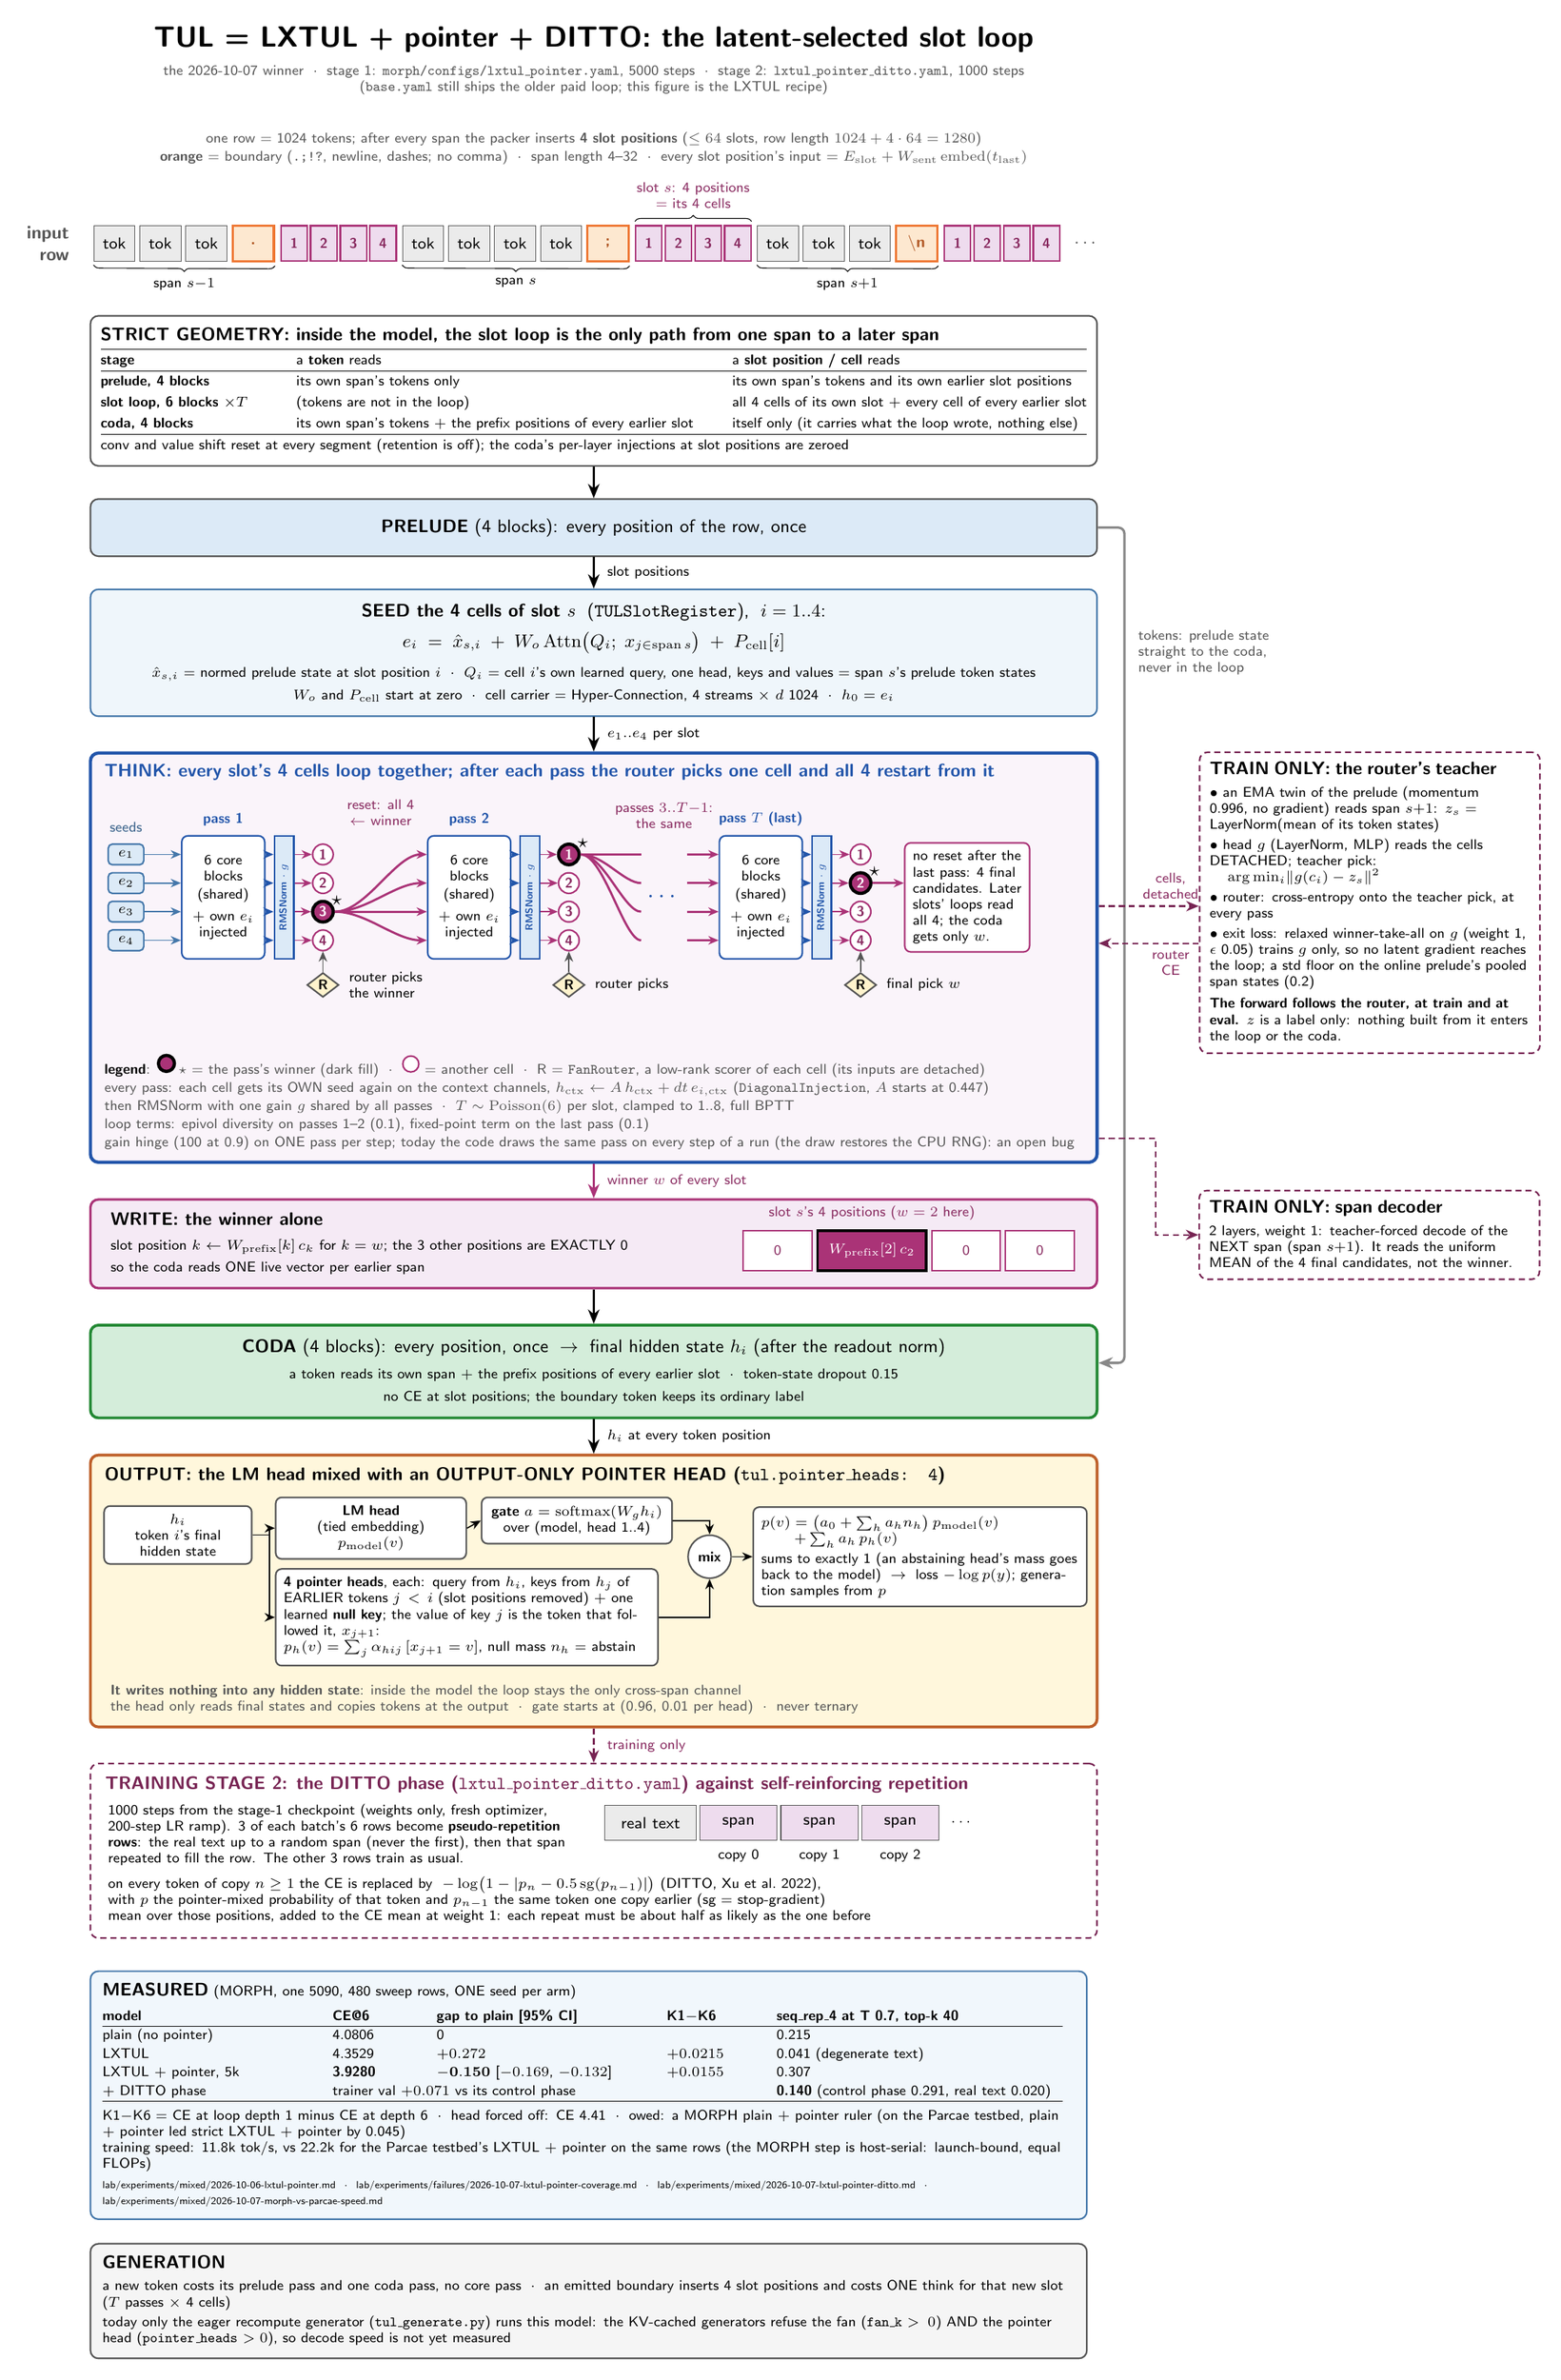
\begin{tikzpicture}[node distance=0.55cm]

% ════════════════════════════════════════════════════════════════════════════
% 1. THE ROW
% ════════════════════════════════════════════════════════════════════════════
\node[tok] (a1) at (0.42, 0) {tok};
\node[tok, right=0.07cm of a1] (a2) {tok};
\node[tok, right=0.07cm of a2] (a3) {tok};
\node[punct, right=0.07cm of a3] (a4) {.};
\node[slot, right=0.09cm of a4] (s11) {1};
\node[slot, right=0.03cm of s11] (s12) {2};
\node[slot, right=0.03cm of s12] (s13) {3};
\node[slot, right=0.03cm of s13] (s14) {4};
\node[tok, right=0.09cm of s14] (b1) {tok};
\node[tok, right=0.07cm of b1] (b2) {tok};
\node[tok, right=0.07cm of b2] (b3) {tok};
\node[tok, right=0.07cm of b3] (b4) {tok};
\node[punct, right=0.07cm of b4] (b5) {;};
\node[slot, right=0.09cm of b5] (s21) {1};
\node[slot, right=0.03cm of s21] (s22) {2};
\node[slot, right=0.03cm of s22] (s23) {3};
\node[slot, right=0.03cm of s23] (s24) {4};
\node[tok, right=0.09cm of s24] (c1) {tok};
\node[tok, right=0.07cm of c1] (c2) {tok};
\node[tok, right=0.07cm of c2] (c3) {tok};
\node[punct, right=0.07cm of c3] (c4) {\textbackslash n};
\node[slot, right=0.09cm of c4] (s31) {1};
\node[slot, right=0.03cm of s31] (s32) {2};
\node[slot, right=0.03cm of s32] (s33) {3};
\node[slot, right=0.03cm of s33] (s34) {4};
\node[font=\small\sffamily, text=bdr, right=0.12cm of s34] {$\cdots$};

\node[ph, text=bdr, left=0.3cm of a1, align=right] {input\\row};

\draw[decorate, decoration={brace, mirror, amplitude=3pt}]
  ($(a1.south west)+(0,-0.06)$) -- ($(a4.south east)+(0,-0.06)$)
  node[midway, below=3pt, sub] {span $s{-}1$};
\draw[decorate, decoration={brace, mirror, amplitude=3pt}]
  ($(b1.south west)+(0,-0.06)$) -- ($(b5.south east)+(0,-0.06)$)
  node[midway, below=3pt, sub] {span $s$};
\draw[decorate, decoration={brace, mirror, amplitude=3pt}]
  ($(c1.south west)+(0,-0.06)$) -- ($(c4.south east)+(0,-0.06)$)
  node[midway, below=3pt, sub] {span $s{+}1$};
\draw[decorate, decoration={brace, amplitude=3pt}]
  ($(s21.north west)+(0,0.06)$) -- ($(s24.north east)+(0,0.06)$)
  node[midway, above=3pt, sub, text=cbPurple!80!black, align=center]
  {slot $s$: 4 positions\\= its 4 cells};

% notation and title above the row
\node[src, anchor=south] (rule) at (8.8, 1.25) {%
  one row = 1024 tokens; after every span the packer inserts \textbf{4 slot positions}
  ($\le 64$ slots, row length $1024 + 4\cdot 64 = 1280$)\\[1pt]
  \textbf{orange} = boundary (\texttt{.;!?}, newline, dashes; no comma) \;$\cdot$\; span
  length 4--32 \;$\cdot$\; every slot position's input $= E_{\mathrm{slot}} + W_{\mathrm{sent}}\,
  \mathrm{embed}(t_{\mathrm{last}})$};
\node[font=\Large\sffamily\bfseries, anchor=south] (title) at ($(rule.north)+(0,1.15)$)
  {TUL = LXTUL + pointer + DITTO: the latent-selected slot loop};
\node[src, anchor=north, align=center] at ($(title.south)+(0,0.02)$)
  {the 2026-10-07 winner \;$\cdot$\; stage 1: \texttt{morph/configs/lxtul\_pointer.yaml}, 5000 steps
  \;$\cdot$\; stage 2: \texttt{lxtul\_pointer\_ditto.yaml}, 1000 steps\\
  (\texttt{base.yaml} still ships the older paid loop; this figure is the LXTUL recipe)};

% ════════════════════════════════════════════════════════════════════════════
% 2. STRICT GEOMETRY: who reads what
% ════════════════════════════════════════════════════════════════════════════
\node[draw=bdr, thick, rounded corners=4pt, fill=white, anchor=north,
      minimum width=17.6cm, inner sep=5pt, font=\scriptsize\sffamily]
  (geo) at (8.8, -1.25) {%
  \renewcommand{\arraystretch}{1.3}%
  \begin{tabular}{@{}>{\bfseries}p{3.0cm} p{7.2cm} p{6.2cm}@{}}
  \multicolumn{3}{@{}l}{\small\bfseries STRICT GEOMETRY: inside the model, the slot loop is
    the only path from one span to a later span}\\[1pt]
  \hline
  stage & a \textbf{token} reads & a \textbf{slot position / cell} reads\\
  \hline
  prelude, 4 blocks & its own span's tokens only &
    its own span's tokens and its own earlier slot positions\\
  slot loop, 6 blocks $\times T$ & (tokens are not in the loop) &
    all 4 cells of its own slot $+$ every cell of every earlier slot\\
  coda, 4 blocks & its own span's tokens $+$ the prefix positions of every earlier slot &
    itself only (it carries what the loop wrote, nothing else)\\
  \hline
  \multicolumn{3}{@{}l}{conv and value shift reset at every segment (retention is off);
    the coda's per-layer injections at slot positions are zeroed}
  \end{tabular}};

% ════════════════════════════════════════════════════════════════════════════
% 3. PRELUDE and SEED
% ════════════════════════════════════════════════════════════════════════════
\node[B, fill=fBlue, below=0.55cm of geo] (pre) {%
  \textbf{PRELUDE} (4 blocks): every position of the row, once};
\draw[A] (geo.south) -- (pre.north);

\node[B, fill=fBlue!45, draw=cbBlue, below=0.55cm of pre, align=center] (seed) {%
  \textbf{SEED the 4 cells of slot $s$} \;(\texttt{TULSlotRegister}), \;$i = 1..4$:\\[4pt]
  $e_i \;=\; \hat x_{s,i} \;+\; W_o\,\mathrm{Attn}\big(Q_i;\; x_{j \in \mathrm{span}\,s}\big)
   \;+\; P_{\mathrm{cell}}[i]$\\[4pt]
  {\scriptsize $\hat x_{s,i}$ = normed prelude state at slot position $i$
  \;$\cdot$\; $Q_i$ = cell $i$'s own learned query, one head, keys and values = span $s$'s
  prelude token states}\\
  {\scriptsize $W_o$ and $P_{\mathrm{cell}}$ start at zero \;$\cdot$\; cell carrier =
  Hyper-Connection, 4 streams $\times$ $d$ 1024 \;$\cdot$\; $h_0 = e_i$}};
\draw[A] (pre.south) -- (seed.north) node[midway, right=3pt, sub] {slot positions};

% ════════════════════════════════════════════════════════════════════════════
% 4. THINK: the latent-selected loop, unrolled
% ════════════════════════════════════════════════════════════════════════════
\node[B, fill=fPurple!30, draw=loopC, line width=1.6pt, minimum height=7.15cm,
      below=0.6cm of seed] (think) {};
\draw[A] (seed.south) -- (think.north) node[midway, right=3pt, sub] {$e_1..e_4$ per slot};
\node[font=\small\sffamily\bfseries, text=loopC, anchor=north west]
  at ($(think.north west)+(0.15,-0.1)$)
  {THINK: every slot's 4 cells loop together; after each pass the router picks one cell and
  all 4 restart from it};

\begin{scope}[shift={($(think.north west)+(0,-2.55)$)}]
  % seeds
  \foreach \r/\yy in {1/0.75, 2/0.25, 3/-0.25, 4/-0.75}
    \node[seed] (e\r) at (0.65, \yy) {$e_{\r}$};
  \node[sub, text=cbBlue!80!black, above=2pt of e1] {seeds};

  \onepass{p1}{2.35}{3}{pass 1}
  \onepass{p2}{6.65}{1}{pass 2}
  \onepass{pT}{11.75}{2}{pass $T$ (last)}

  \foreach \r in {1,2,3,4}
    \draw[As, draw=cbBlue] (e\r.east) -- (p1box.west |- e\r);

  % reset to the winner: winner of pass 1 (cell 3) fans out to all 4 rows of pass 2
  \foreach \yy in {0.75, 0.25, -0.25, -0.75}
    \draw[As, draw=cbPurple, line width=1.1pt] (p1c3.east) .. controls +(0.55,0) and +(-0.55,0)
      .. (p2box.west |- 0,\yy);
  \node[sub, text=cbPurple!80!black, align=center, anchor=south]
    at ($(p1c1.north)!0.5!(p2box.north west)+(0.1,0.12)$)
    {reset: all 4\\$\leftarrow$ winner};

  % pass 2 winner (cell 1) fans out into passes 3..T-1, drawn as stubs + dots
  \coordinate (mid) at ($(p2c1.east)!0.5!(pTbox.west |- p2c1.east)$);
  \foreach \yy in {0.75, 0.25, -0.25, -0.75}
    \draw[draw=cbPurple, line width=1.1pt] (p2c1.east) .. controls +(0.4,0) and +(-0.3,0)
      .. ($(mid |- 0,\yy)+(-0.15,0)$);
  \node[font=\large\sffamily\bfseries, text=loopC] at ($(mid |- 0,0)+(0.25,0)$) {$\cdots$};
  \foreach \yy in {0.75, 0.25, -0.25, -0.75}
    \draw[As, draw=cbPurple, line width=1.1pt] ($(mid |- 0,\yy)+(0.65,0)$) -- (pTbox.west |- 0,\yy);
  \node[sub, text=cbPurple!80!black, align=center, anchor=south]
    at ($(mid |- p2c1.north)+(0.25,0.12)$)
    {passes $3..T{-}1$:\\the same};

  % router labels
  \node[sub, anchor=west, align=left] at ($(p1r.east)+(0.04,0)$) {router picks\\the winner};
  \node[sub, anchor=west, align=left] at ($(p2r.east)+(0.04,0)$) {router picks};
  \node[sub, anchor=west, align=left] at ($(pTr.east)+(0.04,0)$) {final pick $w$};

  % exit, right of the last pass
  \node[draw=cbPurple, thick, rounded corners=3pt, fill=white, font=\scriptsize\sffamily,
        align=left, inner sep=4pt, anchor=west] (exitN) at ($(pTc2.east)+(0.55,-0.25)$)
    {no reset after the\\last pass: 4 final\\candidates. Later\\slots' loops read\\all 4; the coda\\gets only $w$.};
  \draw[As, draw=cbPurple, line width=1.1pt] (pTc2.east) -- (exitN.west |- pTc2);
\end{scope}

% legend + per-pass facts, at the bottom of THINK
\node[src, anchor=south west, align=left, nohyph] (thinkNotes) at ($(think.south west)+(0.15,0.12)$) {%
  {\color{black}\textbf{legend}}: \tikz[baseline=-0.6ex]\node[win, minimum size=0.28cm]{};\,$\star$ = the pass's
  winner (dark fill) \;$\cdot$\; \tikz[baseline=-0.6ex]\node[cell, minimum size=0.28cm]{}; = another cell
  \;$\cdot$\; R = \texttt{FanRouter}, a low-rank scorer of each cell (its inputs are detached)\\[1pt]
  every pass: each cell gets its OWN seed again on the context channels,
  $h_{\mathrm{ctx}} \leftarrow A\,h_{\mathrm{ctx}} + dt\, e_{i,\mathrm{ctx}}$
  (\texttt{DiagonalInjection}, $A$ starts at 0.447)\\[1pt]
  then RMSNorm with one gain $g$ shared by all passes \;$\cdot$\;
  $T \sim \mathrm{Poisson}(6)$ per slot, clamped to 1..8, full BPTT\\[1pt]
  loop terms: epivol diversity on passes 1--2 (0.1), fixed-point term on the last pass (0.1)\\[1pt]
  gain hinge (100 at 0.9) on ONE pass per step; today the code draws the same pass on every
  step of a run (the draw restores the CPU RNG): an open bug};

% ════════════════════════════════════════════════════════════════════════════
% 5. WRITE: the winner only
% ════════════════════════════════════════════════════════════════════════════
\node[B, fill=fPurple!60, draw=cbPurple, line width=1.2pt, minimum height=1.55cm,
      below=0.6cm of think] (write) {};
\draw[A, draw=cbPurple] (think.south) -- (write.north)
  node[midway, right=3pt, sub, text=cbPurple!80!black] {winner $w$ of every slot};
\node[font=\small\sffamily, anchor=west, align=left] (writeT) at ($(write.west)+(0.25,0)$)
  {\textbf{WRITE: the winner alone}\\[1pt]
   {\scriptsize slot position $k$ $\leftarrow$ $W_{\mathrm{prefix}}[k]\,c_k$ for $k = w$;
   the 3 other positions are EXACTLY 0}\\
   {\scriptsize so the coda reads ONE live vector per earlier span}};
\node[slot, minimum width=1.2cm, minimum height=0.7cm, font=\scriptsize\sffamily,
      fill=white, anchor=west] (w1) at ($(write.center)+(2.6,-0.12)$) {0};
\node[slot, minimum width=1.9cm, minimum height=0.7cm, font=\scriptsize\sffamily\bfseries,
      fill=cbPurple, text=white, draw=black, line width=1.4pt, right=0.06cm of w1] (w2)
  {$W_{\mathrm{prefix}}[2]\,c_2$};
\node[slot, minimum width=1.2cm, minimum height=0.7cm, font=\scriptsize\sffamily,
      fill=white, right=0.06cm of w2] (w3) {0};
\node[slot, minimum width=1.2cm, minimum height=0.7cm, font=\scriptsize\sffamily,
      fill=white, right=0.06cm of w3] (w4) {0};
\node[sub, above=1pt of w2, text=cbPurple!80!black] {slot $s$'s 4 positions ($w = 2$ here)};

% ════════════════════════════════════════════════════════════════════════════
% 6. CODA
% ════════════════════════════════════════════════════════════════════════════
\node[B, fill=fTeal, draw=cbTeal, line width=1.4pt, below=0.6cm of write] (coda) {%
  \textbf{CODA} (4 blocks): every position, once \;$\rightarrow$\; final hidden state $h_i$
  (after the readout norm)\\[2pt]
  {\scriptsize a token reads its own span $+$ the prefix positions of every earlier slot
  \;$\cdot$\; token-state dropout 0.15}\\
  {\scriptsize no CE at slot positions; the boundary token keeps its ordinary label}};
\draw[A] (write.south) -- (coda.north);

% tokens skip the loop: prelude state straight to the coda, down the right margin
\coordinate (bypX) at ($(think.east)+(0.45,0)$);
\draw[A, draw=bdr!70, line width=1.2pt, rounded corners=3pt]
  (pre.east) -| (bypX |- seed.south) |- ($(coda.east)+(0,0.15)$);
\node[sub, anchor=west, align=left, text=bdr]
  at ($(bypX |- seed.center)+(0.12,0)$) {tokens: prelude state\\straight to the coda,\\never in the loop};

% ════════════════════════════════════════════════════════════════════════════
% 7. OUTPUT: LM head + the output-only pointer head
% ════════════════════════════════════════════════════════════════════════════
\node[B, fill=fYellow!70, draw=cbOrange!80!black, line width=1.4pt, minimum height=4.75cm,
      below=0.6cm of coda] (ptr) {};
\draw[A] (coda.south) -- (ptr.north) node[midway, right=3pt, sub] {$h_i$ at every token position};
\node[font=\small\sffamily\bfseries, anchor=north west, align=left]
  at ($(ptr.north west)+(0.15,-0.1)$)
  {OUTPUT: the LM head mixed with an OUTPUT-ONLY POINTER HEAD (\texttt{tul.pointer\_heads: 4})};

\begin{scope}[shift={($(ptr.north west)+(0,-0.75)$)}]
  \node[pbox, anchor=north west, text width=2.3cm] (hin) at (0.25, -0.15)
    {\textbf{$h_i$}\\token $i$'s final\\hidden state};
  \node[pbox, anchor=north west, text width=3.05cm] (lmh) at (3.25, 0.0)
    {\textbf{LM head}\\(tied embedding)\\$p_{\mathrm{model}}(v)$};
  \node[pbox, anchor=north west, text width=6.4cm, align=left] (heads) at (3.25, -1.25)
    {\textbf{4 pointer heads}, each: query from $h_i$, keys from $h_j$ of EARLIER tokens
    $j < i$ (slot positions removed) $+$ one learned \textbf{null key}; the value of key $j$
    is the token that followed it, $x_{j+1}$:\\
    $p_h(v) = \sum_j \alpha_{hij}\,[x_{j+1} = v]$, null mass $n_h$ = abstain};
  \node[pbox, anchor=north west, text width=3.05cm] (gate) at (6.85, 0.0)
    {\textbf{gate} $a = \mathrm{softmax}(W_g h_i)$\\over (model, head 1..4)};
  \node[circle, draw=bdr, thick, fill=white, minimum size=0.75cm, font=\scriptsize\sffamily\bfseries]
    (mix) at (10.85, -1.05) {mix};
  \node[pbox, anchor=west, text width=5.55cm, align=left] (pout) at (11.6, -1.05)
    {$p(v) = \big(a_0 + \sum_h a_h n_h\big)\,p_{\mathrm{model}}(v)$\\
    \hspace*{2.2em}$+ \sum_h a_h\,p_h(v)$\\[2pt]
    sums to exactly 1 (an abstaining head's mass goes back to the model) \;$\rightarrow$\;
    loss $-\log p(y)$; generation samples from $p$};
  \draw[As] (hin.east) -- ++(0.3,0) |- (lmh.west);
  \draw[As] (hin.east) -- ++(0.3,0) |- (heads.west);
  \draw[As] (lmh.east) -- (gate.west);
  \draw[As] (gate.east) -| (mix.north);
  \draw[As] (heads.east) -| (mix.south);
  \draw[As] (mix.east) -- (pout.west);
\end{scope}
\node[src, anchor=south west, align=left, nohyph] at ($(ptr.south west)+(0.25,0.12)$) {%
  \textbf{It writes nothing into any hidden state}: inside the model the loop stays the only
  cross-span channel\\
  the head only reads final states and copies tokens at the output \;$\cdot$\; gate starts at (0.96, 0.01 per head) \;$\cdot$\; never ternary};

% ════════════════════════════════════════════════════════════════════════════
% 8. TRAINING STAGE 2: the DITTO phase (dashed: training only)
% ════════════════════════════════════════════════════════════════════════════
\node[B, train, minimum height=3.05cm, below=0.6cm of ptr, inner sep=0pt] (ditto) {};
\draw[Ad, draw=cbPurple!70!black] (ptr.south) -- (ditto.north)
  node[midway, right=3pt, sub, text=cbPurple!80!black] {training only};
\node[font=\small\sffamily\bfseries, anchor=north west, align=left, text=cbPurple!70!black]
  at ($(ditto.north west)+(0.15,-0.1)$)
  {TRAINING STAGE 2: the DITTO phase (\texttt{lxtul\_pointer\_ditto.yaml}) against
  self-reinforcing repetition};
\node[sub, anchor=north west, align=left, text width=8.2cm, nohyph] (dtxt)
  at ($(ditto.north west)+(0.2,-0.6)$)
  {1000 steps from the stage-1 checkpoint (weights only, fresh optimizer, 200-step LR
  ramp). 3 of each batch's 6 rows become \textbf{pseudo-repetition rows}: the real text up
  to a random span (never the first), then that span repeated to fill the row. The other
  3 rows train as usual.};
% a pseudo-repetition row
\begin{scope}[shift={($(ditto.north west)+(9.0,-1.05)$)}]
  \node[tok, minimum width=1.6cm, anchor=west] (r0) at (0,0) {real text};
  \node[tok, minimum width=1.35cm, anchor=west, fill=fPurple, right=0.05cm of r0] (r1) {span};
  \node[tok, minimum width=1.35cm, anchor=west, fill=fPurple, right=0.05cm of r1] (r2) {span};
  \node[tok, minimum width=1.35cm, anchor=west, fill=fPurple, right=0.05cm of r2] (r3) {span};
  \node[sub, right=0.08cm of r3] (r4) {$\cdots$};
  \node[sub, below=1pt of r1] {copy 0};
  \node[sub, below=1pt of r2] {copy 1};
  \node[sub, below=1pt of r3] {copy 2};
\end{scope}
\node[sub, anchor=south west, align=left, nohyph]
  at ($(ditto.south west)+(0.2,0.15)$)
  {on every token of copy $n \ge 1$ the CE is replaced by
  $\;-\log\!\big(1 - \lvert p_n - 0.5\,\mathrm{sg}(p_{n-1})\rvert\big)$ (DITTO, Xu et al.\ 2022),\\
  with $p$ the pointer-mixed probability of that token and $p_{n-1}$ the same token one copy
  earlier (sg = stop-gradient)\\
  mean over those positions, added to the CE mean at weight 1: each repeat must be about half
  as likely as the one before};

% ════════════════════════════════════════════════════════════════════════════
% 9. TRAIN-ONLY HEADS (dashed), right column
% ════════════════════════════════════════════════════════════════════════════
\node[train, anchor=north west, text width=5.6cm] (teach) at ($(think.north east)+(1.75,0)$) {%
  {\small\bfseries TRAIN ONLY: the router's teacher}\\[3pt]
  $\bullet$ an EMA twin of the prelude (momentum 0.996, no gradient) reads span $s{+}1$:
  $z_s$ = LayerNorm(mean of its token states)\\[2pt]
  $\bullet$ head $g$ (LayerNorm, MLP) reads the cells DETACHED; teacher pick:\\
  \hspace*{1.2em}$\arg\min_i \lVert g(c_i) - z_s\rVert^2$\\[2pt]
  $\bullet$ router: cross-entropy onto the teacher pick, at every pass\\[2pt]
  $\bullet$ exit loss: relaxed winner-take-all on $g$ (weight 1, $\epsilon$ 0.05) trains
  $g$ only, so no latent gradient reaches the loop; a std floor on the online prelude's
  pooled span states (0.2)\\[3pt]
  \textbf{The forward follows the router, at train and at eval.} $z$ is a label only:
  nothing built from it enters the loop or the coda.};
\draw[Ad, draw=cbPurple!70!black] ($(think.east)+(0,0.9)$) -- ($(teach.west |- think.east)+(0,0.9)$)
  node[pos=0.72, above, sub, align=center, text=cbPurple!80!black] {cells,\\detached};
\draw[Ad, draw=cbPurple!70!black] ($(teach.west |- think.east)+(0,0.25)$) -- ($(think.east)+(0,0.25)$)
  node[pos=0.28, below, sub, align=center, text=cbPurple!80!black] {router\\CE};

\node[train, anchor=north west, text width=5.6cm] (spandec) at ($(write.north east)+(1.75,0.15)$) {%
  {\small\bfseries TRAIN ONLY: span decoder}\\[3pt]
  2 layers, weight 1: teacher-forced decode of the NEXT span (span $s{+}1$). It reads the
  uniform MEAN of the 4 final candidates, not the winner.};
\draw[Ad, draw=cbPurple!70!black] ($(think.south east)+(0,0.45)$) -- ++(1.0,0) |- (spandec.west);

% ════════════════════════════════════════════════════════════════════════════
% 10. GENERATION and MEASURED
% ════════════════════════════════════════════════════════════════════════════
\node[draw=cbBlue, thick, rounded corners=4pt, fill=fBlue!40, anchor=north west,
      text width=17.0cm, font=\scriptsize\sffamily, align=left, inner sep=6pt, nohyph]
  (meas) at ($(ditto.south west)+(0,-0.55)$) {%
  {\small\bfseries MEASURED} (MORPH, one 5090, 480 sweep rows, ONE seed per arm)\\[3pt]
  \renewcommand{\arraystretch}{1.15}%
  \begin{tabular}{@{}p{3.6cm} p{1.4cm} p{3.6cm} p{1.5cm} p{5.0cm}@{}}
  \textbf{model} & \textbf{CE@6} & \textbf{gap to plain [95\% CI]} & \textbf{K1$-$K6} & \textbf{seq\_rep\_4 at T 0.7, top-k 40}\\
  \hline
  plain (no pointer) & 4.0806 & 0 & & 0.215\\
  LXTUL & 4.3529 & $+0.272$ & $+0.0215$ & 0.041 (degenerate text)\\
  LXTUL $+$ pointer, 5k & \textbf{3.9280} & $\mathbf{-0.150}$ [$-0.169$, $-0.132$] & $+0.0155$ & 0.307\\
  $+$ DITTO phase & \multicolumn{2}{p{5.2cm}}{trainer val $+0.071$ vs its control phase} & & \textbf{0.140} (control phase 0.291, real text 0.020)\\
  \hline
  \end{tabular}\\[3pt]
  K1$-$K6 = CE at loop depth 1 minus CE at depth 6 \;$\cdot$\; head forced off: CE 4.41
  \;$\cdot$\; owed: a MORPH plain $+$ pointer ruler (on the Parcae testbed, plain $+$ pointer
  led strict LXTUL $+$ pointer by 0.045)\\
  training speed: 11.8k tok/s, vs 22.2k for the Parcae testbed's LXTUL $+$ pointer on the same
  rows (the MORPH step is host-serial: launch-bound, equal FLOPs)\\[2pt]
  {\tiny lab/experiments/mixed/2026-10-06-lxtul-pointer.md \;$\cdot$\;
  lab/experiments/failures/2026-10-07-lxtul-pointer-coverage.md \;$\cdot$\;
  lab/experiments/mixed/2026-10-07-lxtul-pointer-ditto.md \;$\cdot$\;
  lab/experiments/mixed/2026-10-07-morph-vs-parcae-speed.md}};

\node[draw=bdr, thick, rounded corners=4pt, fill=fGray!50, anchor=north west,
      text width=17.0cm, font=\scriptsize\sffamily, align=left, inner sep=6pt, nohyph]
  (gen) at ($(meas.south west)+(0,-0.4)$) {%
  {\small\bfseries GENERATION}\\[3pt]
  a new token costs its prelude pass and one coda pass, no core pass \;$\cdot$\; an emitted
  boundary inserts 4 slot positions and costs ONE think for that new slot ($T$ passes
  $\times$ 4 cells)\\[2pt]
  today only the eager recompute generator (\texttt{tul\_generate.py}) runs this model: the
  KV-cached generators refuse the fan (\texttt{fan\_k} $> 0$) AND the pointer head
  (\texttt{pointer\_heads} $> 0$), so decode speed is not yet measured};

\end{tikzpicture}
\end{document}
